% ****** Start of file apssamp.tex ******
%
%   This file is part of the APS files in the REVTeX 4.2 distribution.
%   Version 4.2a of REVTeX, December 2014
%
%   Copyright (c) 2014 The American Physical Society.
%
%   See the REVTeX 4 README file for restrictions and more information.
%
% TeX'ing this file requires that you have AMS-LaTeX 2.0 installed
% as well as the rest of the prerequisites for REVTeX 4.2
%
% See the REVTeX 4 README file
% It also requires running BibTeX. The commands are as follows:
%
%  1)  latex apssamp.tex
%  2)  bibtex apssamp
%  3)  latex apssamp.tex
%  4)  latex apssamp.tex
%
\documentclass[%
 reprint,
%  superscriptaddress,
%groupedaddress,
%unsortedaddress,
%runinaddress,
%frontmatterverbose, 
%preprint,
%preprintnumbers,
%nofootinbib,
%nobibnotes,
%bibnotes,
 amsmath,amssymb,
 aps,
 prl,
%pra,
% prb,
% rmp,
%prstab,
%prstper,
%floatfix,
]{revtex4-2}

\usepackage{graphicx}% Include figure files
\usepackage{dcolumn}% Align table columns on decimal poi<?xml version="1.0" encoding="UTF-8" standalone="no"?>
\usepackage{bm}% bold math
\usepackage{blindtext}
\usepackage{float}
\usepackage{caption,cancel}
\usepackage{cleveref}
\usepackage{subcaption}
\usepackage{xcolor}
%\usepackage{hyperref}% add hypertext capabilities
%\usepackage[mathlines]{lineno}% Enable numbering of text and display math
%\linenumbers\relax % Commence numbering lines

%\usepackage[showframe,%Uncomment any one of the following lines to test 
%%scale=0.7, marginratio={1:1, 2:3}, ignoreall,% default settings
%%text={7in,10in},centering,
%%margin=1.5in,
%%total={6.5in,8.75in}, top=1.2in, left=0.9in, includefoot,
%%height=10in,a5paper,hmargin={3cm,0.8in},
%]{geometry}


\newcommand{\etal}{{\it et al.}~}
\newcommand{\bom}{\boldsymbol{\omega}}

% \newcommand{\sd}[3][\null]{\ensuremath{\dfrac{\d^{#1} #2}{\d #3^{#1}}}}%Standard derivative 
% \newcommand{\pd}[3][\null]{\ensuremath{\dfrac{\partial^{#1} #2}{\partial #3^{#1}}}}%Partial derivative
% \newcommand{\matd}[2][\null]{\ensuremath{\dfrac{\mathrm{D}^{#1} #2}{\mathrm{D} t^{#1}}}} %Material derivative

\def\s{\mathbf{s}}
\def\v{\mathbf{v}}
\def\x{\mathbf{x}}
\def\r{\mathbf{r}}
\def\k{\mathbf{k}}
\def\h{\mathbf{h}}

\def\cm{\mathrm{cm}}
\def\cms{\mathrm{cm/s}}
\def\sec{\mathrm{s}}
\def\K{\mathrm{K}}

\def\red#1{\textcolor{red}{#1}}
\def\blue#1{\textcolor{blue}{#1}}
\def\magenta#1{\textcolor{magenta}{#1}}


% %%%%%%%%%%%%%%%%%%%%%%%%%%%%%%%%%
\newcommand*{\PZS}[1]{\red{#1}} % PZS corrections
\newcommand*{\LG}[1]{{\blue{#1}}}    % LG corrections
\newcommand*{\GK}[1]{{\magenta{#1}}}   % GK corrections


\begin{document}


\preprint{APS/123-QED}

\title{Velocity circulation statistics in counterflow turbulence}

\author{P. Z. Stasiak}
\affiliation{School of Mathematics, Statistics and Physics, Newcastle University, Newcastle upon Tyne, NE1 7RU, United Kingdom}

\author{G. Krstulovic}
\affiliation{Universit\'e C\^ote d'Azur, Observatoire de la C\^ote d'Azur, CNRS,Laboratoire Lagrangre, Boulevard de l'Observatoire CS 34229 - F 06304 NICE Cedex 4, France}

\author{L. Galantucci}
\affiliation{Istituto per le Applicazioni del Calcolo ``M. Picone" IAC CNR, Via dei Taurini 19, 00185 Roma, Italy}

\date{\today}% It is always \today, today,
             %  but any date may be explicitly specified

\begin{abstract}
  \blindtext
\end{abstract}

%\keywords{Suggested keywords}%Use showkeys class option if keyword
   %display desired
\maketitle
 
\section{Introduction}

\blindtext[2]

\section{Method}

Superfluid dynamics are modelled by employing the recently developed \textsc{FOUCAULT} model \cite{galantucci2020}. 
We follow Schwarz's approach \cite{schwarz1988}, by exploiting the large separation of scales between the \textsuperscript{4}He vortex core size $a_0$ and the average inter-vortex spacing $\ell$. 
We parametrize the superfluid vortex lines as 1D space curves $\s(\xi,t)$ with $\xi$ and $t$ the arclength and time respectively. 
The corresponding equation of motion is
$$
\dot{\s}(\xi,t) = \v_{s_{\perp}} + \beta\s'\times(\v_n - \v_s) + \beta'\s'\times\left[\s'\times(\v_n - \v_s)\right]
$$
where $\s'=\partial\s/\partial\xi$ is the unit tangent vector at $\s$, $\v_n$ and $\v_s$ are the normal fluid and superfluid velocities at $\s$, and $\beta$, $\beta'$ are temperature and Reynolds number dependent mutual friction coefficients. The superfluid velocity $\v_s$ is computed via a de-singularized Biot-Savart integral, accelerated using the tree algorithm \cite{baggaley2012d} (see Supplementary Materials). 


\section{Results}


\begin{figure*}
  \centering
  \includegraphics[width=0.99\textwidth]{snapshots.pdf}
  \caption{Visualisation of turbulent vortex tangles. (\emph{a}) Counterflow-induced turbulence generated at $T = 2.1$ K with a counterflow velocity of $v_{ns} = \bar{v}_n - \bar{v}_s = 0.94$ cm/s. The blue and red surface rendering shows the normalised kinetic energy density of normal fluid fluctuations $E'_n/E'_{max}$ where $E'_n = |\v_n - \bar{\v}_n|^2$. (\emph{b}) Turbulence generated by an initial Taylor-Green configuration (see Supplementary Materials for details). In both (\emph{a}) and (\emph{b}) superfluid vortex lines are represented as green tubes with exaggerated size.}

\end{figure*}



\begin{figure}
  \centering
  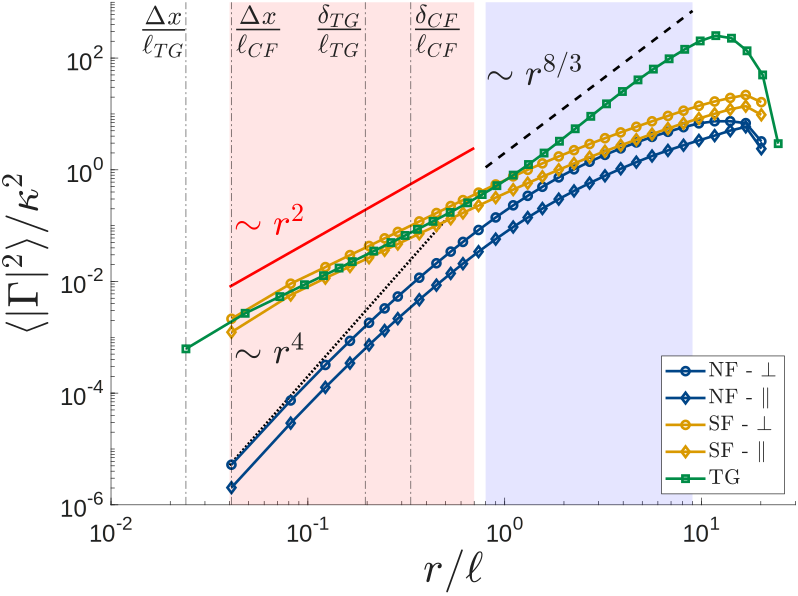
\includegraphics[width=0.49\textwidth]{variance.pdf}
  \caption{Circulation variance $\langle|\Gamma|^2\rangle$ around square loops of size $r$. The blue and yellow curves show the normal fluid and super fluid simulations respectively, which are subdivided into the perpendicular (circles) and parallel (diamonds) components. The green squares show the Taylor-Green simulation.}
  \label{fig:variance}
\end{figure}





\begin{figure}
  \centering
  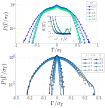
\includegraphics[width=0.49\textwidth]{PDFs.pdf}
  \caption{PDFs of the velocity circulation for different loop sizes $r/\ell > 1$, scaled by the standard deviation $\sigma_{\Gamma}$. (\emph{a}) shows the Taylor-Green simulation, while \emph{(b)} shows both of the normal fluid parallel (diamonds) and perpendicular (circles) components. The inset of (\emph{a}) shows the flatness $\mathcal{K}(\Gamma) = \langle|\Gamma|^4\rangle / \sigma_{\Gamma}^4$, with the same color scheme as in Fig.~\ref{fig:variance}. The black dashed line marks the Gaussian flatness of $\mathcal{K}=3$. }
  \label{fig:PDF}
\end{figure}




\begin{figure}
  \centering
  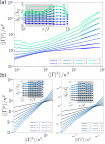
\includegraphics[width=0.49\textwidth]{moments.pdf}
  \caption{Circulation moments $\langle|\Gamma|^p\rangle$ in extended self-similarity (ESS) using $p=3$. (\emph{a}) shows the Taylor-Green simulation, while the left and right panels of (\emph{b}) are the normal fluid perpendicular and parallel component respectively. The insets of each plot give the local slope, where $\lambda_p/\lambda_3 = d\log\langle|\Gamma|^p\rangle/d\log\langle|\Gamma|^3\rangle$ and the horizontal lines correspond to the K41 scalings $\lambda_p^{K41} = 4p/3$. The shaded regions indicate the classical region where the data used to estimate the exponents.}
\end{figure}



\begin{figure}
  \centering
  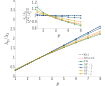
\includegraphics[width=0.49\textwidth]{exponents.pdf}
  \caption{Scaling exponents of velocity circulation moments, estimated within the classical range $r>\ell$. The colour scheme and linestyles is the same as in Fig.~\ref{fig:variance}. The black dashed line represents the self-similar K41 scaling $\lambda_p^{K41} = 4p/3$. The inset shows the proportional deviation from K41 theory.}
\end{figure}



\bibliography{references}

% \begin{acknowledgments}
% \end{acknowledgments}




\end{document}
%
% ****** End of file apssamp.tex ******
